% 第 13 题平面几何图（三角形 + 三等分点）：按固定源 PDF 矢量路径换算（1 pt → 0.03515 cm）。
% 原点取 B 点（源页 (554.98, 317.76) pt），y 向上。
% A 在上、B 左下、C 右下；D 为 BC 中点，E、F 为 AD 三等分点（E 近 A、F 近 D）。
% 自 B、C 分别向 A、E、F 连线（6 条，均在到达目标点前约 3.6–3.8 pt 处收笔，留白给箭头——照源）；
% 另有底边 BC 与中线 AD；A、E、F 三点处各一个实心箭头（指向该点）。
% 直角等几何按源矢量复刻（源内为示意，非严格作图）。
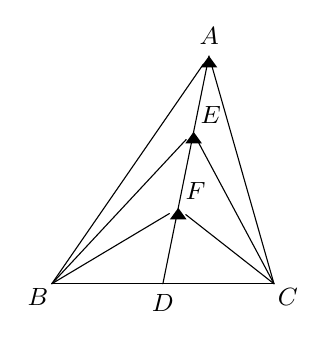
\begin{tikzpicture}[line cap=round,line join=round,font=\small,x=0.03515cm,y=0.03515cm]
% ===== 线段（8 条）=====
\draw (0,0)--(80.26,0);            % B–C（底边）
\draw (0,0)--(54.76,79.35);        % B–A
\draw (80.26,0)--(57.78,78.85);    % C–A
\draw (40.13,0)--(56.79,82.30);    % D–A（中线）
\draw (0,0)--(48.57,52.13);        % B–E
\draw (80.26,0)--(52.70,51.59);    % C–E
\draw (0,0)--(42.48,25.37);        % B–F
\draw (80.26,0)--(48.40,24.99);    % C–F
% ===== 箭头（3 处，各一个实心三角形，指向 A/E/F）=====
\fill (56.79,82.30)--(53.79,78.15)--(59.79,78.15)--cycle;   % → A
\fill (51.24,54.87)--(48.24,50.72)--(54.24,50.72)--cycle;   % → E
\fill (45.68,27.43)--(42.68,23.28)--(48.68,23.28)--cycle;   % → F
% ===== 标注（照源字框中心，显式坐标）=====
\node[anchor=center,inner sep=0] at (56.84,89.44) {\(A\)};
\node[anchor=center,inner sep=0] at (-4.99,-4.93) {\(B\)};
\node[anchor=center,inner sep=0] at (85.33,-4.93) {\(C\)};
\node[anchor=center,inner sep=0] at (40.07,-6.98) {\(D\)};
\node[anchor=center,inner sep=0] at (57.40,61.08) {\(E\)};
\node[anchor=center,inner sep=0] at (51.96,33.53) {\(F\)};
\end{tikzpicture}
